\documentclass[14pt,margin=0.5in,innermargin=0in,blockverticalspace=-0.1in,colspace=-1.0cm]{tikzposter}
\geometry{paperwidth=841mm,paperheight=594mm}
\usepackage[utf8]{inputenc}
\usepackage{lmodern}
\usepackage{anyfontsize}
\usepackage{csquotes}
\usepackage{amsmath}
\usepackage{amsfonts}
\usepackage{amsthm}
\usepackage{amssymb}
\usepackage{mathrsfs}
\usepackage{graphicx}
\usepackage{adjustbox}
\usepackage{enumitem}
\usepackage{xcolor}
\usepackage[backend=biber,style=numeric,sorting=none]{biblatex}
\usepackage{durham-theme}
\usepackage{mwe} % for placeholder images
\usepackage{tcolorbox}
\usepackage{multicol}

\usepackage{caption}
\captionsetup[figure]{font=large,labelfont=bf}

\addbibresource{references.bib}

% set theme parameters
\tikzposterlatexaffectionproofoff
\usetheme{DurhamTheme}
\usecolorstyle{DurhamStyle}

\usepackage[scaled]{helvet}
\renewcommand\familydefault{\sfdefault} 
\renewcommand{\vec}[1]{\bm{#1}}
\newcommand{\Tr}{\text{Tr}}
\usepackage[T1]{fontenc}

\title{Megapixel Image Generation with Step-unrolled Denoising Autoencoders}
\author{\textbf{Alex F. McKinney}\textsuperscript{1},
\textbf{Chris G. Willcocks}\textsuperscript{1,2} 
}
\institute{\textsuperscript{1}Department of Computer Science, Durham University\\
            \textsuperscript{2}Project Supervisor
            }
\titlegraphic{\includegraphics[width=0.16\linewidth]{durham-logo.png}}

% begin document
\begin{document}
\maketitle

\centering
\block{}
{
    \vspace{-2.5cm}
    \centering
    \begin{tikzfigure}
        
\includegraphics[width=1.0\linewidth]{samples.png}
    \end{tikzfigure}
    \captionof{figure}{
            \centering
            $1024 \times 1024$ samples from our FFHQ1024 model. Resulting
            samples are diverse and of high-fidelity. Each sample was generated
            in $\approx 2$ seconds on a consumer-grade GPU (GTX 1080Ti), in
            contrast to existing approaches at this resolution, which take
            minutes to generate. To our knowledge, this is the fastest sampling,
            non-adversarial generative framework at this resolution.
        }
    \vspace{0.5cm}
    \begin{scope}[line width=\titlelinewidth,]
    \draw[color=colorOne!30!colorOne,round cap-round cap]
    (\titleposleft,0)--(100,0);
    \end{scope}
}

\begin{columns}

    \column{0.3}
    \block{}{
        \vspace{-1cm}
        \begin{tcolorbox}[boxsep=0pt,top=0cm,bottom=1.1cm,adjusted title={\Large\bf
            Background},colbacktitle=colorOne]
        \begin{tikzfigure}
            \includegraphics[width=1.0\linewidth]{AR-NAR.pdf}
        \end{tikzfigure}
        \vspace{-0.5cm}
        \captionof{figure}{
                Autoregressive sampling (left) is defined in terms of the
                probabilistic chain rule, so sampling is done iteratively with
                complexity $\mathcal{O}(n)$. Non-autoregressive sampling (right)
                can sample an arbitrary number of elements in parallel, so
                number of steps does not scale with input size. It can also use
                the full context available to it, resulting in better quality
                samples and flexible inpainting. However, existing NAR methods
                still typically require many network evaluations to produce
                meaningful samples.
                %Autoregressive sampling (left) is defined in terms of the
                %probabilistic chain rule, meaning that sampling is done
                %iteratively -- one element at a time -- so not to violate
                %causality. Non-autoregressive sampling (right) does not have
                %such constraints, and can sample an arbitrary number of elements
                %in parallel. Crucially, this means the iteration complexity of
                %sampling does not scale directly with data dimensionality, allowing
                %massive scaleability. In addition, it can use the full context
                %available to it, in order to make predictions, allowing for
                %better quality samples and more flexible inpainting. Despite
                %such advantages, non-adversarial, non-autoregressive generative
                %models have not seen widespread adoption, due to requiring
                %many sampling steps -- potentially thousands.
            }
        
        \vspace{-1cm}

        \begin{tikzfigure}
            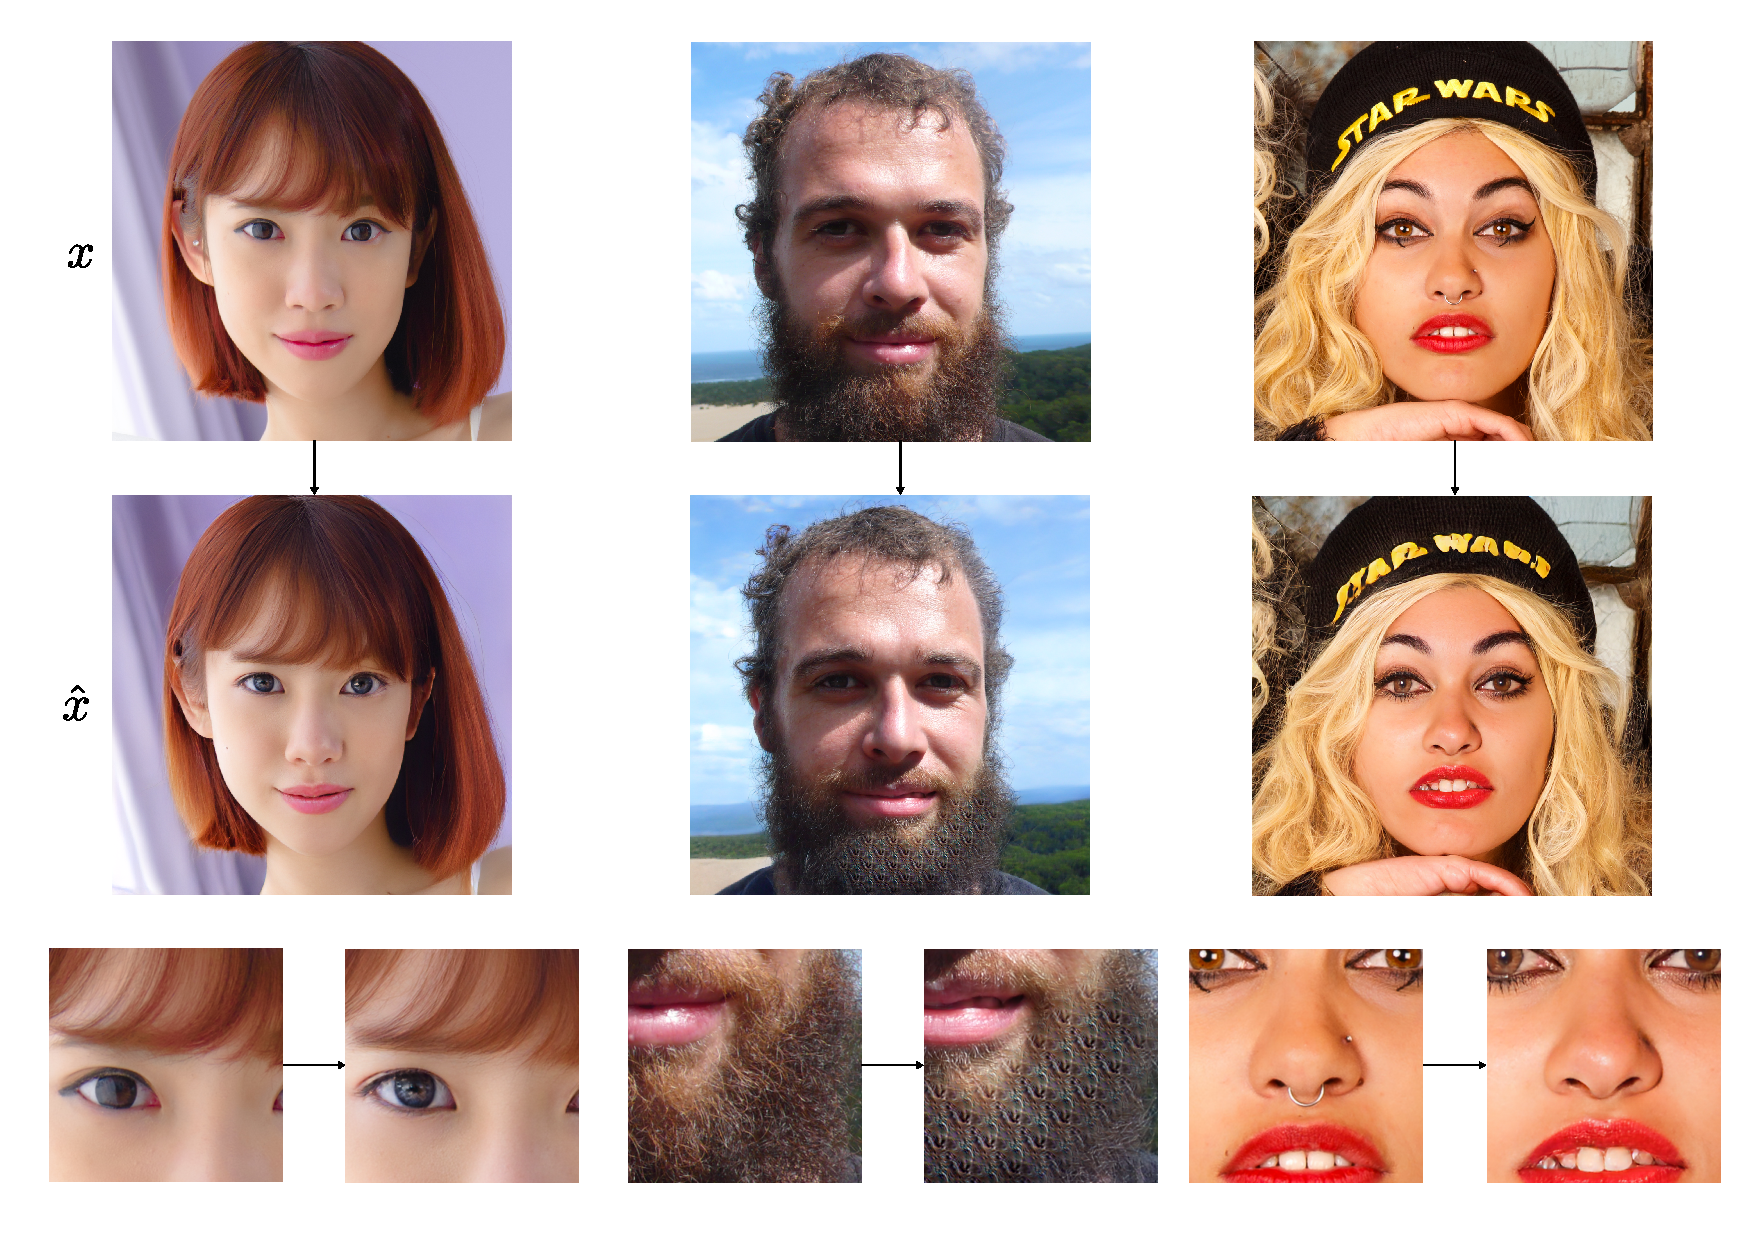
\includegraphics[width=0.99\linewidth]{recon.pdf}
        \end{tikzfigure}
        \vspace{-1.0cm}
        \captionof{figure}{
                VQ-GAN is used to reduce computational requirements for training
                and sampling of generative models by acting as a compression
                model. VQ-GAN does not always faithfully reproduce the input
                image, though outputs are perceptually valid. For example, left
                shows a change in eye colour and the concealment of a piercing
                by adjusting hair position. Middle has its hair texture changed.
                Right has piercings removed and text corruption.
            }
            
        \end{tcolorbox}
    }
    
    \column{0.4}
    \block{}{
        \vspace{-1cm}
        \begin{tcolorbox}[boxsep=0pt,top=0cm,adjusted title={\Large\bf Proposed Method},colbacktitle=colorOne]
        \begin{tikzfigure}
            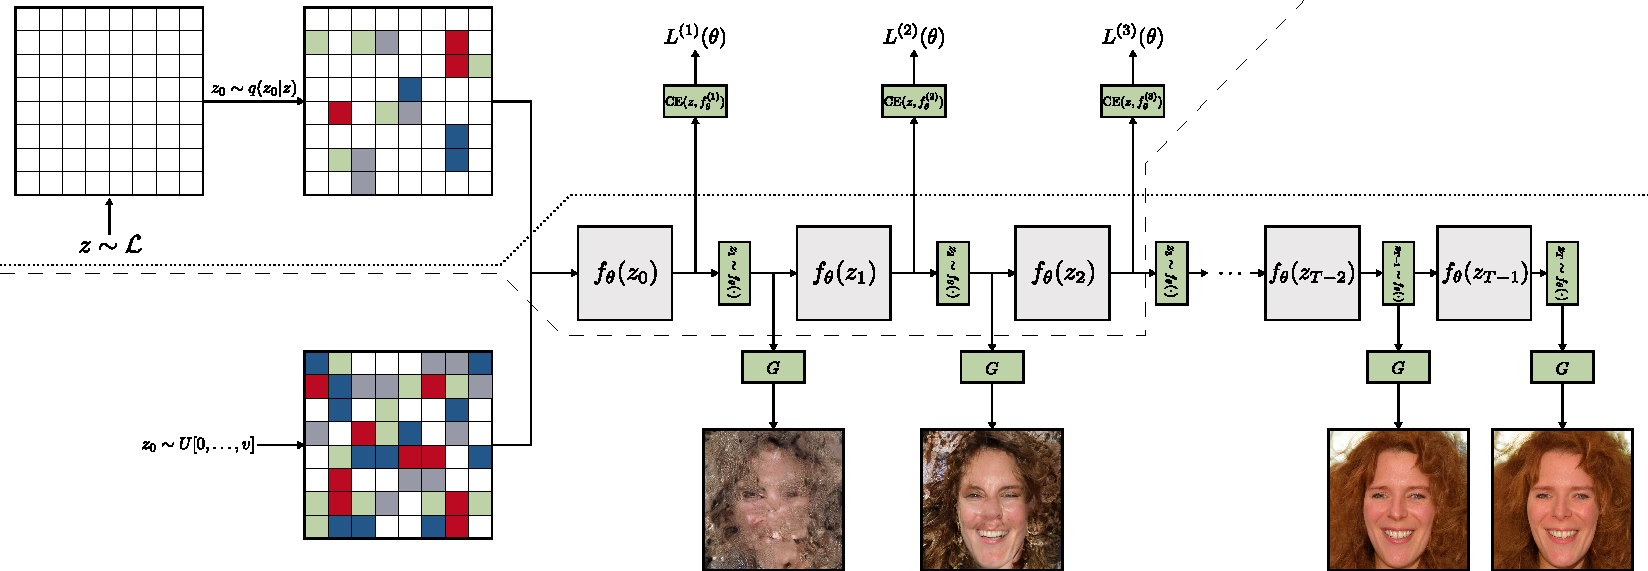
\includegraphics[width=0.99\linewidth]{overall.pdf}
        \end{tikzfigure}
        \vspace{-0.5cm}
        \captionof{figure}{
                An overview of the SUNDAE training and sampling of discrete
                latent representations. Above the dashed line represents the
                process for training, whereas below the dotted line represents
                the sampling process. The training process begins by sampling
                $\mathbf{z} \sim \mathcal{L}$ and then sampling from the
                corruption distribution $q(\mathbf{z}_0 \vert \mathbf{z})$.
                SUNDAE then denoises for 2 to 3 steps, computing the
                cross-entropy loss at each step in the chain which is
                subsequently averaged to produce a final loss. Sampling begins
                by obtaining $\mathbf{z}_0$ from a uniform prior and iteratively
                denoising. SUNDAE easily outspeeds prior autoregressive and
                (non-adversarial) non-autoregressive models, using typically
                50-100 steps ($\approx$ 2 seconds) during sampling.
            }
        \vspace{-0.6cm}

        \begin{minipage}{0.40\linewidth}
            \begin{align*}
            \begin{split}
                L_\text{PIX} &= \alpha_\text{PIX} \cdot |\mathbf{x} -
                \hat{\mathbf{x}}| \cdot \\
                L_\text{GAN} &= \alpha_\text{GAN} \cdot \left(\log D(\mathbf{x}) + \log
                (1-D(\hat{\mathbf{x}}))\right) \\
                L &= L_\text{VQ} + \lambda \cdot L_\text{GAN}
            \end{split}
            \end{align*}
        \end{minipage}
        \begin{minipage}{0.59\linewidth}
            \begin{align*}
            \begin{split}
                L_\text{VQ} &= \alpha_\text{VQ} \cdot \left(||\hat{\mathbf{z}} -
                \mathbf{z}||^2 + ||sg[E(\mathbf{x})] - \mathbf{z}||^2_2 +
                ||E(\mathbf{x}) -
                sg[\mathbf{z}]||^2_2\right)\\
                \lambda &= \frac{\nabla_{G_{-1}}[L_\text{PIX} +
                L_\text{PER}]}{\nabla_{G_{-1}}[L_\text{GAN}] + \epsilon}\\
                \alpha_\text{PIX} &= 1.0,\; \alpha_\text{VQ} = 1.0,\; \alpha_\text{GAN} = 0.5,\; \alpha_\text{PER} = 1.0
            \end{split}
            \end{align*}
        \end{minipage}
        \vspace{0.4cm}

        \textbf{Equation 1:} Loss function for our VQ-GAN model trained on $1024
        \times 1024$ images.
        \vspace{0.3cm}

        %\begin{align}
        %\begin{split}
            %L_\text{PIX} &= \alpha_\text{PIX} \cdot |\image - \hat{\image}| \cdot \\
            %L_\text{VQ} &= \alpha_\text{VQ} \cdot \left(||\hat{\latent} -
            %\latent||^2 + ||sg[\vqganEncoder(x)] - \latent||^2_2 + ||\vqganEncoder(x) -
            %sg[\latent]||^2_2\right)\\
            %L_\text{GAN} &= \alpha_\text{GAN} \cdot \left(\log D(x) + \log
            %(1-D(\hat{x}))\right) \\
            %\lambda &= \frac{\nabla_{G_{-1}}[L_\text{PIX} +
            %L_\text{PER}]}{\nabla_{G_{-1}}[L_\text{GAN}] + \epsilon}\\
            %L &= L_\text{VQ} + \lambda \cdot L_\text{GAN}\\
            %\alpha_\text{PIX} &= 1.0,\; \alpha_\text{VQ} = 1.0,\; \alpha_\text{GAN} = 0.5,\; \alpha_\text{PER} = 1.0
        %\end{split}
        %\end{align}

        \large
        The objective of this project was to push the efficiency of generative
        models to their limit and expand the array of non-autoregressive methods
        for image generation. By combining various methods -- each at the
        pinnacle of efficiency in their respective areas. These include VQ-GAN, a
        vector quantization model with an unparalleled rate of compression;
        hourglass transformers, a highly scaleable attention model; and SUNDAE,
        a fast, non-autoregressive text generative model.

        Our primary contributions are as follows:
        \begin{itemize}
            \item
                The development of a non-autoregressive, non-adversarial
                generative modelling framework with extremely flexible sampling
                and capabilities for self-correction, self-stopping, conditional
                generation, and arbitrary inpainting patterns. The model can be
                directly configured for both low- and high-step sampling
                scenarios, resulting in high quality and diverse samples in 
                seconds of sampling time.

            \item
                Addressing flaws in the original formulation of SUNDAE and
                hourglass transformers to be more suited for the modelling of
                multi-dimensional discrete data. Though applied to discrete
                latents in our work, the modifications are also applicable in a
                wider context, such as to pixel-level modelling. We also
                demonstrate the superiority of hierarchical transformers --
                forming a key component in the scalability of our approach. 

            \item
                The scaling of VQ-GAN to extremely high resolution ($1024 \times
                1024$) images of human faces. This resolution far exceeds
                resolutions achieved in prior work with VQ-GAN. This allowed for
                the \textbf{generation of megapixel images in as few as two
                seconds} on a consumer-grade GPU when combined with our fast and
                scalable generative framework. This is in contrast to prior
                autoregressive methods and non-autoregressive diffusion methods
                that take minutes to generate, or cannot scale to such
                resolutions entirely.

        \end{itemize}
        \end{tcolorbox}
    }

    \column{0.3}
    \block{}{
        \vspace{-1cm}
        \begin{tcolorbox}[boxsep=0pt,top=0cm,bottom=1.0cm,adjusted title={\Large\bf Results},colbacktitle=colorOne]
        \begin{tikzfigure}
            \includegraphics[width=0.49\linewidth]{imagenet-lakeside.png}
            \hfill
            \includegraphics[width=0.49\linewidth]{imagenet-valley.png}
            \captionof{figure}{
                $256 \times 256$ class-conditioned samples on ImageNet. The left
                batch of samples are from the class ``Lakeside'' whereas the
                right batch are from the class ``Valley''. We note, that our
                approach can be extended to use text prompts as a conditioning
                signal, yielding a text-to-image model.
            }
        \end{tikzfigure}
        
        \vspace{-1cm}

        \begin{tikzfigure}
            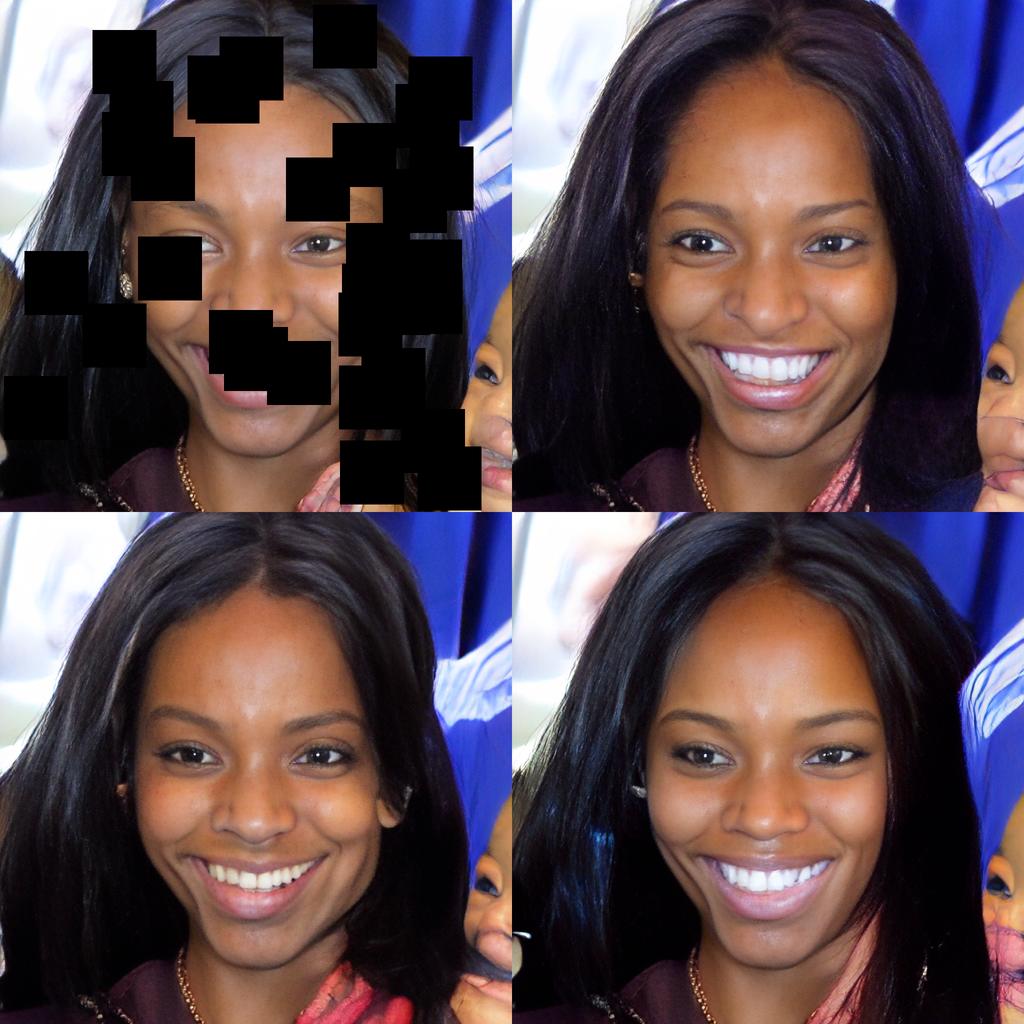
\includegraphics[width=0.49\linewidth]{inpaint-rand.png}
            \hfill
            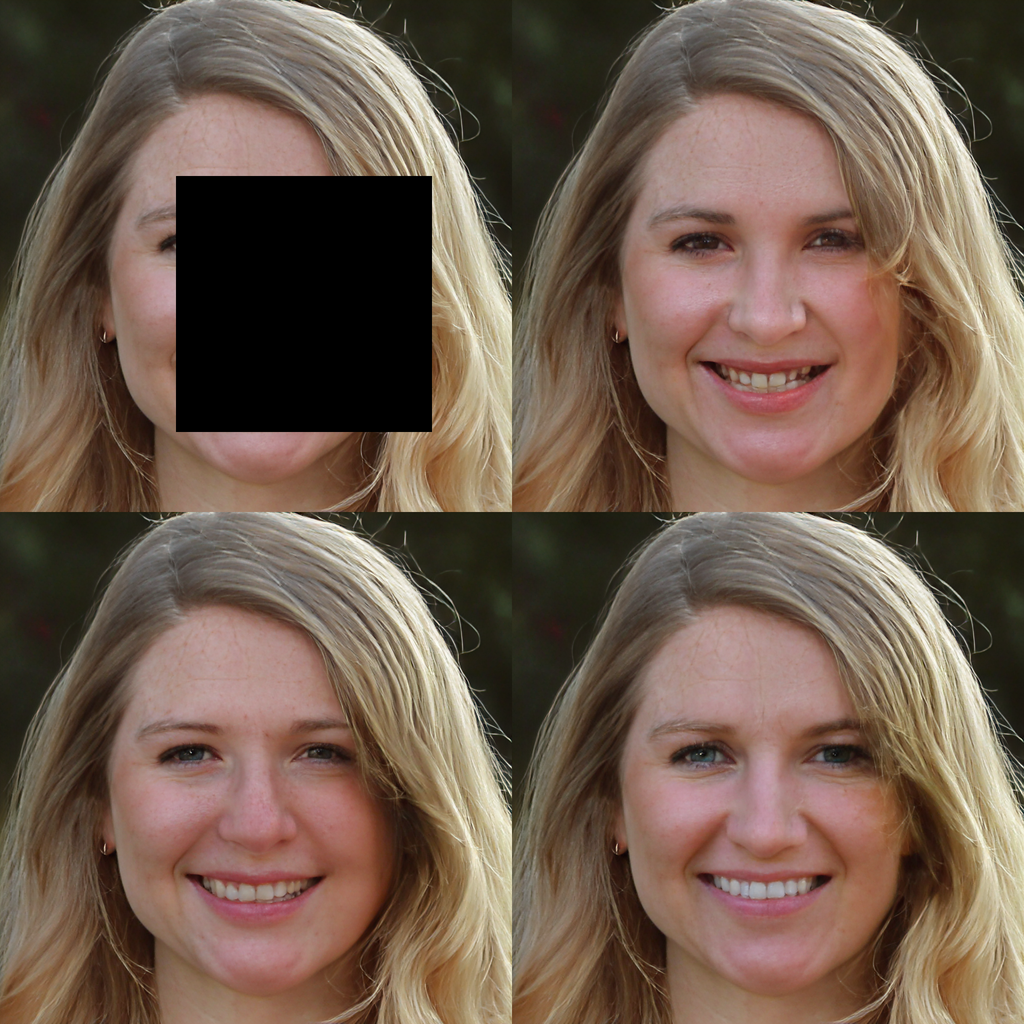
\includegraphics[width=0.49\linewidth]{inpaint-block.png}
            \captionof{figure}{
                Representative inpainting results on FFHQ1024 using our trained
                model. We demonstrate the superiority of NAR
                methods for inpainting by using arbitrary inpainting masks,
                including completely random (left) and large block masks
                (right). Such patterns are difficult to inpaint with using 
                autoregressive models, and cannot utilise the full context
                available to them.
            }
        \end{tikzfigure}
        \end{tcolorbox}
    }

    % TODO: potentially a manual bibliography of relevant literature
    \block{}{
        \vspace{-1cm}
        \begin{tcolorbox}[boxsep=0pt,top=0cm,adjusted title={\Large
            References},colbacktitle=colorOne]
        \nocite{*}
        \vspace{0.4cm}
        \begin{footnotesize}
        \printbibliography[heading=none]
        \end{footnotesize}
        \end{tcolorbox}
    }
\end{columns}
\end{document}
